\chapter{Performance des outils de détection}
\label{lab:chapCAD}
	\section{Généralités}

En oncologie, la détection des sites tumoraux est une étape capitale dans la prise en charge des patients. 
Dans cette partie, je vais détailler les techniques qui permettent de comparer les performances de plusieurs observateurs (médecins ou algorithmes) face aux mêmes images, ou alors du même observateur face à plusieurs types d'images différentes.

Pour cette section, le problème va être simplifié au cas où un observateur doit classer un signal en ``Sain'' (normal, HO) ou ``Pathologique'' (anormal, H1). 

Les performances d'un classifieur sont indiquées par la matrice de confusion (table~\ref{tab:confusion}), qui recense les signaux correctement et incorrectement classés 

\begin{table}[h]
	\label{tab:confusion}
	\begin{tabular}{cc c|c|}
		& & \multicolumn{2}{c}{Classe estimée} \\
		\cline{3-4}	
		& & \multicolumn{1}{|c|}{Sain} & Pathologique \\ 
		\cline{2-4}
		\multicolumn{1}{c|}{\multirow{2}{*}{Classe réelle}} & \multicolumn{1}{|c|}{Sain} & VN (\emph{Vrai Négatif}) & FP (\emph{Faux Positif})\\
		\cline{2-4}
		\multicolumn{1}{c|}{} & \multicolumn{1}{|c|}{Pathologique} & FN (\emph{Faux Négatif}) & VP (\emph{Vrai Positif})\\
		\cline{2-4}
	\end{tabular}
	\caption[Matrice de confusion]{Matrice de confusion : donne une vue
d'ensemble des performances du classifieur. Elle indique le résultat de la
classification de signaux connus.}
\end{table}

On utilise habituellement deux grandeurs pour mesurer les performances d'un classifieur :

La \emph{sensibilité} (voir l'équation~\ref{eq:sensib}) correspond à la proportion d'images correctement évaluées pathologiques par l'observateur par rapport au nombre total d'images réellement pathologiques. Elle donne une information sur la capacité du classifieur à détecter les cas pathologiques.
\label{lab:pressensib}
\begin{equation}
	\label{eq:sensib}
	Sensibilit\acute{e} = \frac{VP}{VP + FN}
\end{equation}

La \emph{spécificité} (voir équation~\ref{eq:specif}) représente le même type de grandeur, mais cette-fois ci appliquée aux cas non pathologiques : elle correspond à la capacité du classifieur à donner un résultat négatif lorsque l'image est non pathologique.

\begin{equation}
	\label{eq:specif}
	Sp\acute{e}cificit\acute{e} = \frac{VN}{VN + FP}
\end{equation}

Ces deux grandeurs sont complémentaires mais ne permettent pas à elle seules de comparer des classifieurs. En effet, un  utilisateur va souvent donner des notes, qui vont indiquer son niveau de confiance sur la présence de la pathologie (à ne pas confondre avec des notations sur la gravité des lésions, comme les techniques de gradation de~\cite{genestie1998comparison}).

Les techniques de comparaison de systèmes de décision comme l'analyse ROC (Receiver-Operating Curve) permettent de prendre en compte ces incertitudes. Elles proviennent à l'origine du domaine des télécommunications pendant la seconde guerre mondiale, où il fallait une métrique permettant de tester les performances des systèmes RADAR~\cite{zou2007receiver} pour la détection des avions ennemis. Les courbes ROC servent donc à évaluer la capacité d'un ou plusieurs ``observateurs'' à discriminer des signaux entre deux classes ``normal'' et ``anormal''. Les informations de sensibilité et de spécificité se limitent à comparer les performances pour un niveau de confiance donné.

\subsection{Définition d'un Vrai positif / Faux positif}

En général, les systèmes CAD génèrent des cartes paramétriques, sur lesquels les voxels ou des groupements de voxels reçoivent une valeur correspondant à leur classe. 

Afin de déterminer si l'élément (voxel ou groupement de voxels) noté ``anormal'' fait effectivement partie d'une lésion, sa  position est généralement comparée à celle des lésions de la vérité terrain. Une distance d'acceptation est utilisée pour prendre en compte une éventuelle imprécision du système CAD. Par exemple, l'auteur de~\cite{paik2004surface} considère que l'élément est un vrai positif si il est contenu dans la tumeur de la vérité terrain.

Cependant, il existe plusieurs stratégies pour compter les FP :
\begin{itemize}
 \item Par voxel ou groupe de voxel (3D)
 \item Par coupe (2D)
\end{itemize}

Ces deux techniques vont très fortement influer sur le nombre de faux positifs pour le même système CAD. En effet, dans le cas où le comptage des FP est réalisé sur l'ensemble de l'image, chaque groupement ou voxel ne correspondant pas à une lésion est noté FP. L'auteur de~\cite{paik2004surface} indique par exemple 165 faux positifs par images TDM pour une sensibilité de 100\%. De même,~\cite{zhao2003automatic} montre une sensibilité de 94\% avec 906 faux positifs par image TDM pour la détection du cancer du poumon. Ces résultats montrent des nombre de faux positifs très importants, mais ne peuvent pas être comparés avec ceux utilisant un chiffrage des FP par coupe. En effet, dans ce cas, ``FP'' correspond au nombre de coupes contenant au moins un élément n'étant pas une tumeur. Le nombre de faux positifs est donc borné par le nombre de coupes, et ne fait pas de différences entre des coupes contenant un grand nombre de lésions et celles n'en contenant qu'une. 

\textbf{Dans le reste du document, nous considèrerons le premier système de comptage des Faux positifs : tout élément du volume à observer n'étant pas en contact avec une tumeur sera compté comme un faux positif.}


	\section{Méthodologie ROC - Receiver-Operating Curve}

Les courbes ROC~\cite{swets1982evaluation,metz1986roc} sont des courbes indiquant la spécificité et la sensibilité de l'observateur (humain ou numérique) pour différents niveaux de certitude. Elles fournissent une mesure objective des performances d'un observateur dans une tâche de discrimination entre deux classes. 

Elles peuvent être utilisées pour comparer les performances relatives de différents observateurs ou pour déterminer leurs paramètres optimaux. L’évaluation d'un observateur par la méthode ROC nécessite la création d'un jeu de données labellisées en deux classes : Normale (H0) et Pathologiques (H1). L'observateur va se voir présenter l'ensemble des images et devra les noter individuellement selon un barème défini à l'avance (par exemple 0: pas du tout pathologique, 1: potentiellement pathologique, 2: équivoque, 3: potentiellement pathologique, 4: définitivement pathologique). Par convention, plus la note (notée $\lambda$) sera élevée, plus l'observateur va considérer qu'il est en présence d'un cas pathologique. A l'inverse, une note basse va indiquer un cas présumé sain. 


\begin{figure}[h]
	\begin{center}
	
\includegraphics[width=10cm]{images/illustrationROC}
%	\vspace{-0.5cm} % Ugly Moche Hideux
	\end{center}
	\caption[Exemple de courbe ROC]{Exemple de courbe ROC. La courbe $A$ représente le résultat d'une évaluation ROC avec un barème à 6 niveaux. Pour chaque note du barème, le point correspondant est affiché en reportant la spécificité et la sensibilité (représentés par les croix). La courbe $B$ représente une autre évaluation, avec des performances inférieures : Pour chaque niveau de ``1-Spécificité'', la sensibilité de la courbe $B$ est inférieure à celle de la courbe $A$. Le courbe $C$ représente le d'un classifieur qui donne ses réponses de manière aléatoire.}
	\label{fig:illustrationROC}
\end{figure}

L'observateur peut être un humain ou un algorithme, et les notes peuvent être discrètes ou continues. 

Le tracé de la courbe ROC se fait en reportant la sensibilité et la valeur "1-spécificité" du classifieur pour différents seuils de décision. Par construction, la courbe va commencer au point $(0,0)$ (tous les points sont diagnostiqués négatifs) et se terminer au point de coordonnée $(1,1)$ (tous les points sont diagnostiqués positifs). Deux exemples de courbes ROC sont présentés sur la figure~\ref{fig:illustrationROC}.


Pour analyser les courbes ROC, on considère que les distributions de probabilité des notes des cas H0 et H1 suivent une loi gaussienne (voir figure~\ref{fig:loiROC}). Ce modèle de décision suppose que l'ensemble des valeurs de $\lambda$ évaluées sur des cas H0 (sain) suit une distribution de probabilité $P(\lambda_0, \sigma_0)$ de valeur moyenne $\lambda_0$ et d'écart-type $\sigma_0$. De même, les valeurs de $\lambda$ évaluées sur des cas H1 (pathologiques), suivent une distribution de probabilité $P(\lambda_1, \sigma_1)$. Le mécanisme de décision se base sur le choix d'une valeur de seuil $\lambda_s$ au-delà de laquelle les observations sont considérées comme pathologiques.

Ce seuil permet de modifier de manière dynamique la répartition des observations dans la matrice de confusion.  Cela permet d'enrichir la comparaison des observateurs par rapport au couple (sensibilité/spécificité) seul.

Selon cette hypothèse gaussienne, on peut montrer que la distance $d$, appelée indice de détectabilité, correspond à l'aire sous la courbe ROC :


\begin{equation}
 d= \frac{d_1 - d_0}{\sqrt{\sigma_1 + \sigma_0}}
\end{equation}

\begin{figure}[h]
	\begin{center}
	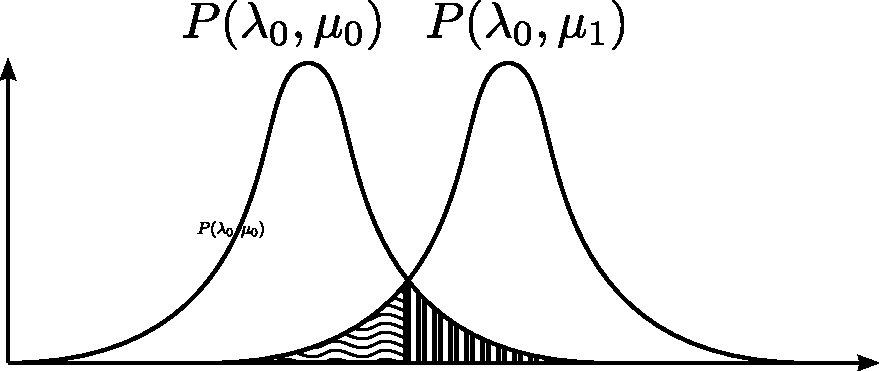
\includegraphics[width=10cm]{images/loiROC}
	\vspace{-0.5cm} % Ugly Moche Hideux
	\end{center}
	\caption[Modèle de la distribution de probabilité de la variable de décision]{Modèle de la distribution de probabilité de la variable de décision dans pour les populations H0 ($P(\lambda_0, \mu_0)$) et H1 ($P(\lambda_1, \mu_1)$) dans les études ROC. $\lambda_s$ représente le seuil à partir duquel une observation sera catégorisée H0 ou H1.}
	\label{fig:loiROC}
\end{figure}




Un ensemble d'indicateurs et de figures de mérite (FDM) permettent de comparer les performances de classifieurs à partir des courbes ROC. La FDM la plus simple consiste à choisir un niveau de spécificité (noté $\alpha$) et à comparer les sensibilités des différents classifieurs. L'avantage de ce système est qu'il permet de comparer les performances dans des conditions proches de la réalité, où l'on cherche à rester dans un taux de spécificité donné. Cependant, les résultats vont dépendre du paramètre $\alpha$. Une métrique plus globale est l'aire sous la courbe ROC. \'Etant donné que la courbe est nécessairement comprise dans un carré unitaire, la valeur de l'aire sera comprise entre 0 (le classifieur donne systématiquement les mauvaises réponses), 0.5 (le classifieur donne des réponses aléatoires) et 1 (le classifieur donne toujours la bonne réponse)~\cite{nie2006integrating}.

Il est important, lors du calcul de la FDM, d'avoir une estimation de l'erreur. Il est possible de l'estimer en ajustant une courbe théorique (répondant à la loi théorique de la figure~\ref{fig:loiROC}). Plusieurs logiciels ont été développés pour estimer les paramètres, qui ont été comparés dans la publication~\cite{CarstenStephan03012003} (AccuROC, Analyse-It, CMDT, GraphROC, MedCalc, mROC, ROCKIT, and SPSS).

\label{lab:p-valeur}
Une grandeur souvent utilisée dans la littérature pour évaluer la pertinence d'un résultat est la \emph{p-valeur}. Elle représente la probabilité d'obtenir des différences entre deux courbes au moins aussi extrême que la différence observée (dans notre cas, les courbes ROC), en prenant en compte l'hypothèse selon laquelle le classifieur est aléatoire. Elle permet de vérifier si le test est statistiquement significatif.

Le problème de la méthodologie ROC est que l'observateur ne donne pas d'information de localisation de la pathologie dans l'image. On lui présente une image et il doit la noter sans indiquer la localisation de la zone suspecte. Dans notre cas, nous voulons comparer des classifieurs qui détectent les tumeurs dans l'image. Il faut non seulement savoir si des lésions sont présentes, mais aussi avoir leur nombre et leur localisation. Cela est proche du travail en routine clinique, qui consiste à évaluer l'étendue et le nombre des lésions pour déterminer l'efficacité d'un traitement par exemple. 

Pour éviter cette limitation, plusieurs extensions à la méthodologie ROC sont décrites dans la littérature : L-ROC, AF-ROC ou encore F-ROC. Les L-ROC sont décrites ci-après, tandis que les AF-ROC et F-ROC seront décrites dans la section suivante.

\subsection{Courbes ``Localization ROC'' (L-ROC)}

L'analyse L-ROC~\cite{farquhar1999roc} ajoute l'information de localisation lors de la décision. L'observateur doit indiquer sur l'image qu'il considère comme pathologique la localisation de la lésion la plus probable. Elle est considérée comme un vrai positif si la distance entre la localisation indiquée et la localisation réelle de la lésion est inférieure à une certaine distance.

Cependant, bien que cette technique prenne en compte l'information de localisation, elle ne permet pas de traiter de manière satisfaisante les cas de lésions multiples.


\section{Courbes Free ROC}	

Les courbes Free-ROC permettent de prendre en compte plus d'informations que les courbes vues précédemment car elles utilisent non seulement les informations de localisation, mais prennent aussi en compte le concept de faux positifs de manière plus approfondie, avec la possibilité d'avoir à la fois des faux positifs et des vrais positifs dans une même image.

\subsection{Courbes Free-ROC}
\label{lab:FROC}

Les courbes F-ROC~\cite{bunch1978free} sont une généralisation des courbes ROC aux cas où l'on évalue la capacité de l'observateur à détecter un ensemble de lésions dans une série d'images. Chaque image pouvant contenir un nombre indéfini de lésions. L'observateur va donc devoir pointer sur l'image l'ensemble des sites suspects et y associer une note.

Dans ce cas, on ne peut pas utiliser le formalisme ROC car le terme de spécificité n'est pas directement calculable pour chaque niveau de confiance. On utilise à sa place le nombre moyen de faux positifs par image pour un seuil donné (voir figure~\ref{fig:courbeFROC}).

On utilise les termes de LL (Lésion localisée) et NL (Non-Lésion) en lieu et place des informations de vrai positifs et faux positifs sur les courbes ROC. De la même manière, la sensibilité et la spécificité sont respectivement FLL (Fraction de lésions correctement détectées et localisées) et NFM (Nombre de faux positifs moyens par image).


\begin{figure}[h]
	\begin{center}
	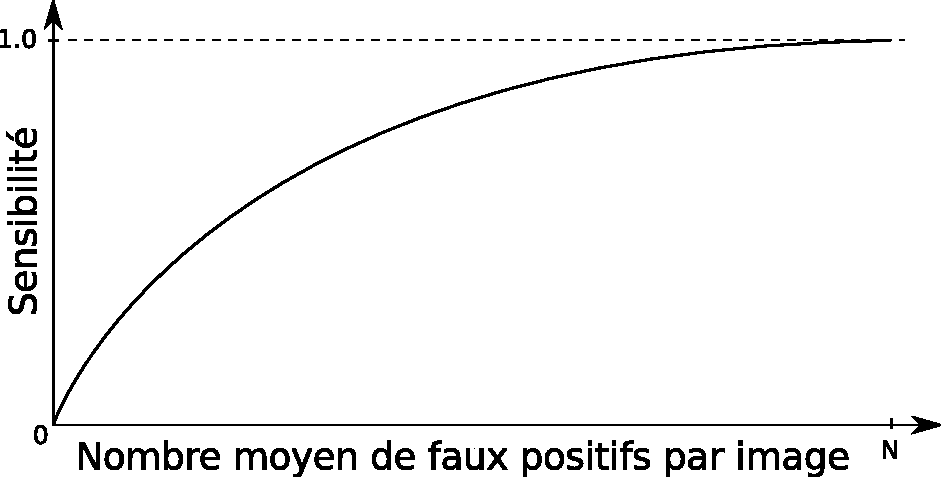
\includegraphics[width=15cm]{images/FROC}
	\end{center}
	\caption{Exemple de courbe Free ROC}
	\label{fig:courbeFROC}
\end{figure}

Les courbes F-ROC n'ayant pas de bornes sur l’axe des abscisses, il est impossible de comparer plusieurs courbes à partir de l'aire sous la courbe. Il reste cependant possible de comparer la sensibilité pour un nombre de faux positifs donnés, mais on retrouve les mêmes problèmes que pour l'analyse ROC : il faut choisir un paramètre.

\subsection{Courbes Alternative Free-ROC}

Les courbes A-FROC~\cite{chakraborty1990free} sont des extensions des courbes Free-ROC présentées précédemment mais qui ne prennent en compte que le faux positif de plus haut score par image, ce qui ne pénalise pas le cas où un observateur indique un grand nombre de fausses détections (NL). On se retrouve alors dans la situation de courbes bornées sur l'axe des abscisses, ce qui permet leur comparaison.

\subsection{Comparaison des courbes}
\label{lab:AFROC}
Plusieurs techniques ont été développées pour permettre de réaliser des comparaisons de courbes dérivées de la méthodologie F-ROC. De la même manière que pour les courbes ROC, il est possible de comparer les courbes F-ROC en fonction de la FLL pour un nombre de faux positifs donnés. Cependant, étant donné que les courbes F-ROC n'ont pas de fin déterminée, il n'est pas possible d'utiliser l'aire sous la courbe. 

JAFROC~\cite{chakraborty2004observer} (JAcknife Free Receiver Operating Curve) est un algorithme et un logiciel développé par Chakraborty et se base sur une FDM non liée directement à la courbe. Cette mesure de performance utilise un algorithme dérivé des études A-FROC, ce qui signifie qu'il n'utilise pas l'ensemble des informations disponibles dans les courbes F-ROC mais se borne à comparer les scores des faux positifs de plus forte note pour chaque image avec les notes des vrais positifs. La figure de mérite $\Theta_J$ proposée mesure la probabilité d'avoir un score de vrai positif supérieur à celui d'un faux positif (de n'importe quelle image).

Soit $\theta_J$ la valeur de la FDM, $N_T$ le nombre total d'images, indexées par $i$, $N_A$ le nombre total de cas pathologiques, indexées par $j$. $n_j$ est le nombre total de lésions dans le cas anormal $j$.

\begin{equation}
\label{eq:JAFROC1}
\begin{array}{l}
	\displaystyle \theta=\frac{1}{N_T N_A} \sum_{i=1}^{N_T} \sum_{j=1}^{N_A} \sum_{k=1}^{n_j} W_{jk} \psi(X_i, Y_{jk}) \\
	\\
	\displaystyle \psi(X,Y) = \left\{
		\begin{array}{lll}
			1.0 & \mbox{si} & Y > X \\
			0.5 & \mbox{si} & Y = X    \\
			0.0 & \mbox{si} & Y < X    \\
		\end{array}
	\right. \\
	\\
	\displaystyle \mbox{avec} \sum_{k=1}^{n_j} W_{jk} = 1 \\
\end{array}
\end{equation}

$X_i$ le score du plus haut faux positif de l'image $i$, $Y_{jk}$ est la note de la lésion k de l'image j. Si une lésion n'a pas été détectée, alors sa note sera par défaut de "0".

Les poids $W_{jk}$ correspondent à l'importance relative de détecter la lésion $k$ dans l'image $j$ pour le diagnostic. Pour chaque image, la somme des poids doit être égale à 1.

Une seconde version de JAFROC existe avec une puissance statistique plus importante, mais elle nécessite de disposer d'un grand nombre de cas non pathologiques. La formule est la même que la précédente (équation~\ref{eq:JAFROC1}). La seule différence est que la première sommation se fait sur l'ensemble des cas non pathologiques $N_N$ (équation~\ref{eq:JAFROC2}) au lieu de l'ensemble des cas $N_T$.

\begin{equation}
\label{eq:JAFROC2}
\theta=\frac{1}{N_T N_A} \sum_{i=1}^{N_N} \sum_{j=1}^{N_A} \sum_{k=1}^{n_j} W_{jk} \psi(X_i, Y_{jk})
\end{equation}


\chapter{Systèmes de détection}

\section{Principe des CAD}

\subsection{Introduction}

Les systèmes CAD (Computer-Aided-Detection) sont des algorithmes permettant d'assister le praticien dans la détection des lésions ou le classement des images médicales. Dans le cadre de l'imagerie TEP oncologique, le besoin principal est celui du suivi thérapeutique, pour lequel, il est important de détecter d'éventuelles lésions résiduelles. Pour cela, il faut que le système CAD soit particulièrement adapté à la recherche de petites lésions de faible contraste qui pourraient échapper au médecin. Cependant, le diagnostic, qui consiste à évaluer la dangerosité des lésions, et leur caractère pathologique est une tâche plus complexe qui relève plus des systèmes d'aide au diagnostic, qui ne seront pas traités ici.

Le développement des systèmes CAD a débuté dans les années 1980~\cite{chan1987image}, notamment pour détecter les micro-calcifications en mammographie. Bien qu'il existe plusieurs systèmes CAD commerciaux pour l'imagerie TDM (xLNA pour Philips par exemple), aucun CAD commercial pour la TEP n'existe à notre connaissance.

\'Etant donné que les systèmes d’aide à la détection dédiées à l’imagerie TEP restent limitées,  le travail de cette thèse s’est largement inspiré de la méthodologie suivie lors du développement de systèmes CAD dans d’autres modalités d’imagerie médicale et particulièrement la mammographie et l’imagerie TDM. La classification supervisée permet de profiter de la disponibilité \textit{a priori} d’images préalablement classées pour fournir un ‘superviseur’ efficace et paramétrable. Le paragraphe suivant définit les différentes étapes standardisées d’un système CAD supervisé.


\subsection{Les différentes étapes d’un système CAD supervisé}

Comme rappelé dans la publication~\cite{li2007recent}, un système CAD est constitué de deux étapes majeures : l’identification initiale des tumeurs et la réduction de faux positifs. 

L’objectif de l’identification initiale des tumeurs (figure \ref{fig:presSystemesCAD}.1),2) et 3)) est de localiser les structures potentiellement suspectes de l’image avec la plus grande sensibilité possible au coût d’un grand nombre de fausses détections. Différents choix méthodologiques doivent être précisés pour cette étape :


\begin{figure}[h]
	\begin{center}
	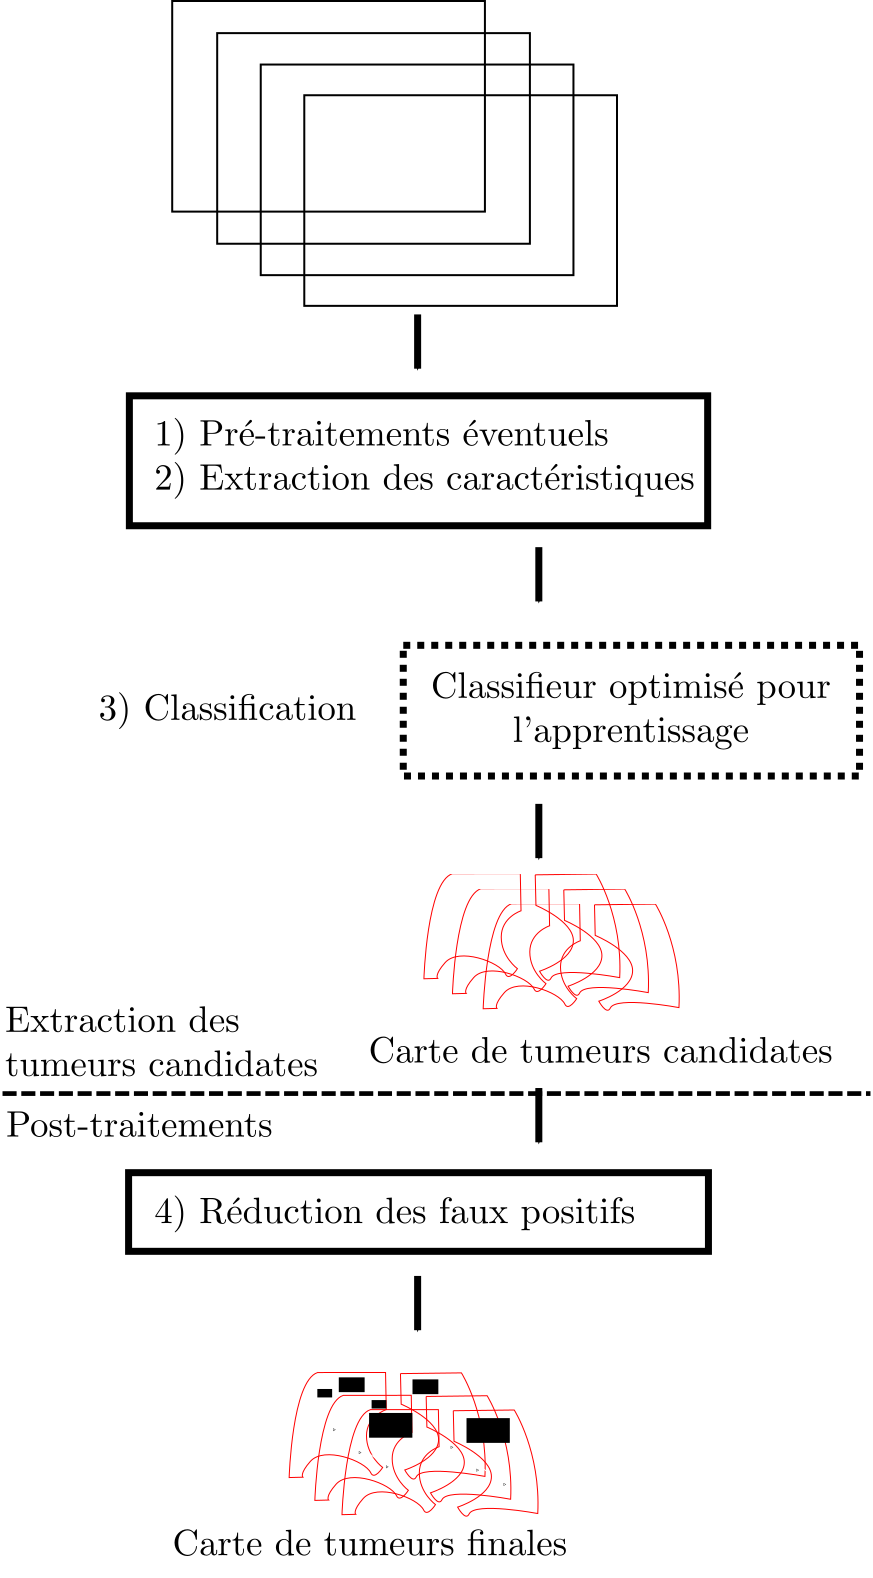
\includegraphics[width=12cm]{images/principeCAD}
	\end{center}
	\caption{Les différentes étapes d'un système CAD}
	\label{fig:presSystemesCAD}
\end{figure}


\begin{itemize}
\item Les régions ou organes d’intérêt du système, lorsque celui-ci n’est pas dédié au corps entier, peuvent être séparés. L’image ou les régions d’intérêt de l’image peuvent ensuite être améliorées lors d’une étape de pré-traitement, reposant par exemple sur du rehaussement du contraste ou du débruitage (figure \ref{fig:presSystemesCAD}.1) ).
\item Le processus d’extraction des tumeurs suspectes passe ensuite par l’utilisation d’un système de classification (figure \ref{fig:presSystemesCAD}.3) )., optimisé par un apprentissage, s’appliquant sur un ensemble de caractéristiques de l’image ou de la structure cible (figure \ref{fig:presSystemesCAD}.2) ). Ce dernier a pour but de déterminer la classe, « tumeur présente » ou « tumeur absente », de l’image ou de la structure cible. 
\item L’objectif de l’étape de réduction de faux positifs (figure \ref{fig:presSystemesCAD}.4) ) est de fortement réduire les fausses détections extraites de l’étape précédente, tout en conservant une sensibilité élevée. Cette étape rassemble un ensemble de méthodes permettant de trier les tumeurs candidates précédemment extraites afin de ne conserver que les candidats les plus ‘suspects’.  
\end{itemize}

	\section{Les CAD en TEP}


Quelques systèmes CAD sur des images TEP ont été décrits dans des travaux académiques, tels que~\cite{guan2006automatic}, qui recherche des anomalies dans le corps entier. Cependant, ils ne donnent pas de mesures de performances quantitatives. La publication de~\cite{kanakatte2008pulmonary} utilise des systèmes de classification supervisés (K plus proches voisins et SVM décrits en~\ref{lab:SVM}). Un seuillage est réalisé, puis les candidats sont classés en utilisant des caractéristiques fréquentielles et les moments statistiques. 

Certaines publications utilisent seulement l'imagerie fonctionnelle TEP~\cite{ying2004novel, kanakatte2007pilot, kanakatte2008pulmonary, saradhi2009framework, el2009exploring, mhd2010artificial}, tandis que d'autres combinent cette information avec l'imagerie TDM~\cite{jafar2006computerized, nie2006integrating, potesil2007automated}.

La plupart des travaux réalisés dans le domaine ont portés sur la segmentation de lésions pré-sélectionnées pour réaliser de l'estimation de volume pour de la planification de radio-thérapie ou du suivi thérapeutique~\cite{kanakatte2007pilot, potesil2007automated, kanakatte2008pulmonary, yu2009automated}. Des publications récentes se sont focalisées sur la problématique du diagnostique pour la classification de nodules~\cite{nie2006integrating} ou la prédiction d'évolution des lésions suite à un traitement~\cite{el2009exploring}. Cependant, très peu d'études se sont focalisées sur la problématique de la localisation des lésions~\cite{guan2006automatic, kanakatte2007pilot, kanakatte2008pulmonary, mhd2010artificial}, surtout dans le cas de lésions de faibles diamètre/faible contraste~\cite{ying2004novel, jafar2006computerized, saradhi2009framework}.

Les systèmes de classifications existants se concentrent en général sur la délimitation de lésions de fort contraste, ce qui ne correspond pas à notre problématique de détection. 


\section{Extraction initiale des lésions}

	\subsection{Pré-traitements de l'image}

Cette étape (figure \ref{fig:presSystemesCAD}.1) ) a pour objectif de préparer et améliorer l’image initiale à l’extraction des tumeurs candidates. 

Cette étape n'est pas obligatoire et certaines études utilisent simplement l’image original en imagerie TDM~\cite{mougiakakou2007differential}. D’autres modifient l’image initiale, pour améliorer les performances finales de classification. En imagerie TDM, des méthodes de rehaussement de contraste sont mises en place à partir de filtres sélectifs~\cite{li2003selective}. Certains pré-traitements visent à éliminer des structures gênantes (vaisseaux sanguins dans les poumons…). En mammographie, il est également courant de débruiter les images par des techniques de filtrage~\cite{bazzani2001svm}. Cependant, le filtrage doit être correctement optimisé pour les images à traiter, car il peut être à l'origine d'une baisse de sensibilité~\cite{ge2005computer}.
	
	\subsection{Extraction des caractéristiques}

Un système de classification ne traite que très rarement directement les voxels de l’image brute. Différentes caractéristiques descriptives de l’image ou du cas clinique (patient) (figure \ref{fig:presSystemesCAD}.2) ) sont utilisées pour réaliser la classification. Celles-ci sont en effet porteuses d’informations plus pertinentes facilitant leur interprétation. Ces caractéristiques sont assimilées à l'analyse réalisée par l'oeil humain avant avant de réaliser le diagnostic sur la présence ou non de tumeurs. Elles sont l’interprétation de l’image d’un point de vue numérique. Elles doivent permettre au classifieur de discriminer les éléments pathologiques des éléments sains et être caractéristiques de chacune des classes. 

Un état de l'art des différentes caractéristiques a été présenté par~\cite{cheng2006approaches}, classées selon leurs catégories. On peut différentier plusieurs familles de caractéristiques selon leur type :

\begin{description}
\item[les régions d’intérêt de l’image :] Que ce soit en imagerie anatomique ou fonctionnelle, les tumeurs apparaissent visuellement avec un degré de distinction variable par rapport au fond de l’organe d’appartenance. Dans le cas de la mammographie et de la TEP au 18F-FDG, les tumeurs sont de captation généralement plus élevée que le tissu environnant. L’imagerie TEP associée à d’autres radiotraceurs que le 18F-FDG peut aussi être caractérisée par un hyposignal dans les tumeurs. Dans le cas de la TDM, les tumeurs correspondent à des nodules de forme spécifique (ellipsoïde) et d’atténuation plus élevée. Etant donné que les tumeurs peuvent, dans certains cas, être caractérisées par la valeur même des pixels ou voxels les constituant, certaines études utilisent directement les voxels de la région d'intérêt comme caractéristiques d’image.
\item[les caractéristiques statistiques : ] Les caractéristiques statistiques reflètent généralement les propriétés de bruit et de texture des zones étudiées. Les statistiques du premier ordre caractérisent les niveaux de gris de l’image sans prendre en compte leur distribution relative. Des mesures de moyennes ou d’histogrammes peuvent être extraites. Les statistiques d’ordre deux représentent généralement des propriétés de texture. Celle-ci est assimilée à l’apparence locale de l’image, c’est à dire l’organisation des détails d’une petite partie de l’image telle que le système visuel humain l’aperçoit.
\item[les caractéristiques cliniques : ] Ce sont les données contenues dans le dossier médical du patient qui peuvent être utilisées comme critère par le système de détection.
\item[les caractéristiques fréquentielles :] Selon~\cite{sachs1971spatial}, le système visuel humain traite l’information à travers des canaux sélectifs en fréquence. Il est ainsi possible de se rapprocher d’une modélisation assez fiable du système visuel humain en se basant sur les caractéristiques fréquentielles des images cibles.
\item[les caractéristiques géométriques :] Les caractéristiques géométriques des tumeurs, exprimées par exemple par des critères de convexité, peuvent aussi être discriminantes. Elles sont généralement simples à interpréter car elles correspondent aux détails visuels sur lesquels se focalisent consciemment les cliniciens. Cette famille de caractéristiques est généralement dédiée aux imageries de type anatomique étant donné qu’elle repose sur une délinéation précise des structures étudiées. Le principal inconvénient des caractéristiques de forme est d’être fortement corrélé à la segmentation initiale des tumeurs étudiées.
\end{description}



	\section{Méthodes de classification}
\todo{sur-sous apprentissage}

Dans cette section je vais décrire les deux principales classes de techniques de classification : supervisée et non supervisée.


		\subsection{Méthodes non supervisées}

Dans le système de classification non supervisée, le classifieur reçoit directement l'ensemble des données à traiter, sans informations supplémentaires. Il devra de lui-même les classer par similitude en groupes. On utilise ce type de classifieur si on ne connaît pas \textit{a priori} les classes, comme présenté dans la figure~\ref{fig:fonctionnementClassifNonSup}. Le nombre de classes peut être un des paramètres d'entrée notamment pour les k-moyennes, ou être déterminé de manière automatique.


La classification non supervisée repose sur une méthode statistique utilisant une fonction de proximité. Toutes les observations d'une même classe devront être proches au sens de cette fonction. Le partitionnement idéal est obtenu lorsque la covariance intraclasse est minimisée, ce qui implique que les classe sont le plus homogènes possible, et que la distance entre les classes est maximisée, pour que les classes soient le plus différenciées possible.

Plusieurs algorithmes sont décrits dans la littérature pour réaliser des classifications non supervisées :

\begin{description}
 \item[K-moyennes (K-means) : ]  c'est un algorithme itératif qui associe à chaque point la classe dont le barycentre est le plus proche, puis remet à jour le centre des classes à la prochaine itération~\cite{herwig1999large}. Cet algorithme nécéssite de fixer le nombre de classes \textit{a priori}.
 \item[Cartes auto-adaptatives : ] Cet algorithme utilise des techniques dérivées des graphes pour partitionner les données~\cite{kohonen1982self}.
 \item[Regroupement ascendant hiérarchique : ] Cet algorithme utilise une mesure de dissimilarité pour regrouper les observations. A la première itération, chaque observation dispose de sa propre classe. A chaque itération suivante, les deux classes contenant les observations les plus proches vont être regroupées, jusqu'à obtenir la classification finale~\cite{ward1963hierarchical}.
\end{description}


\begin{figure}[h]
	\begin{center}
	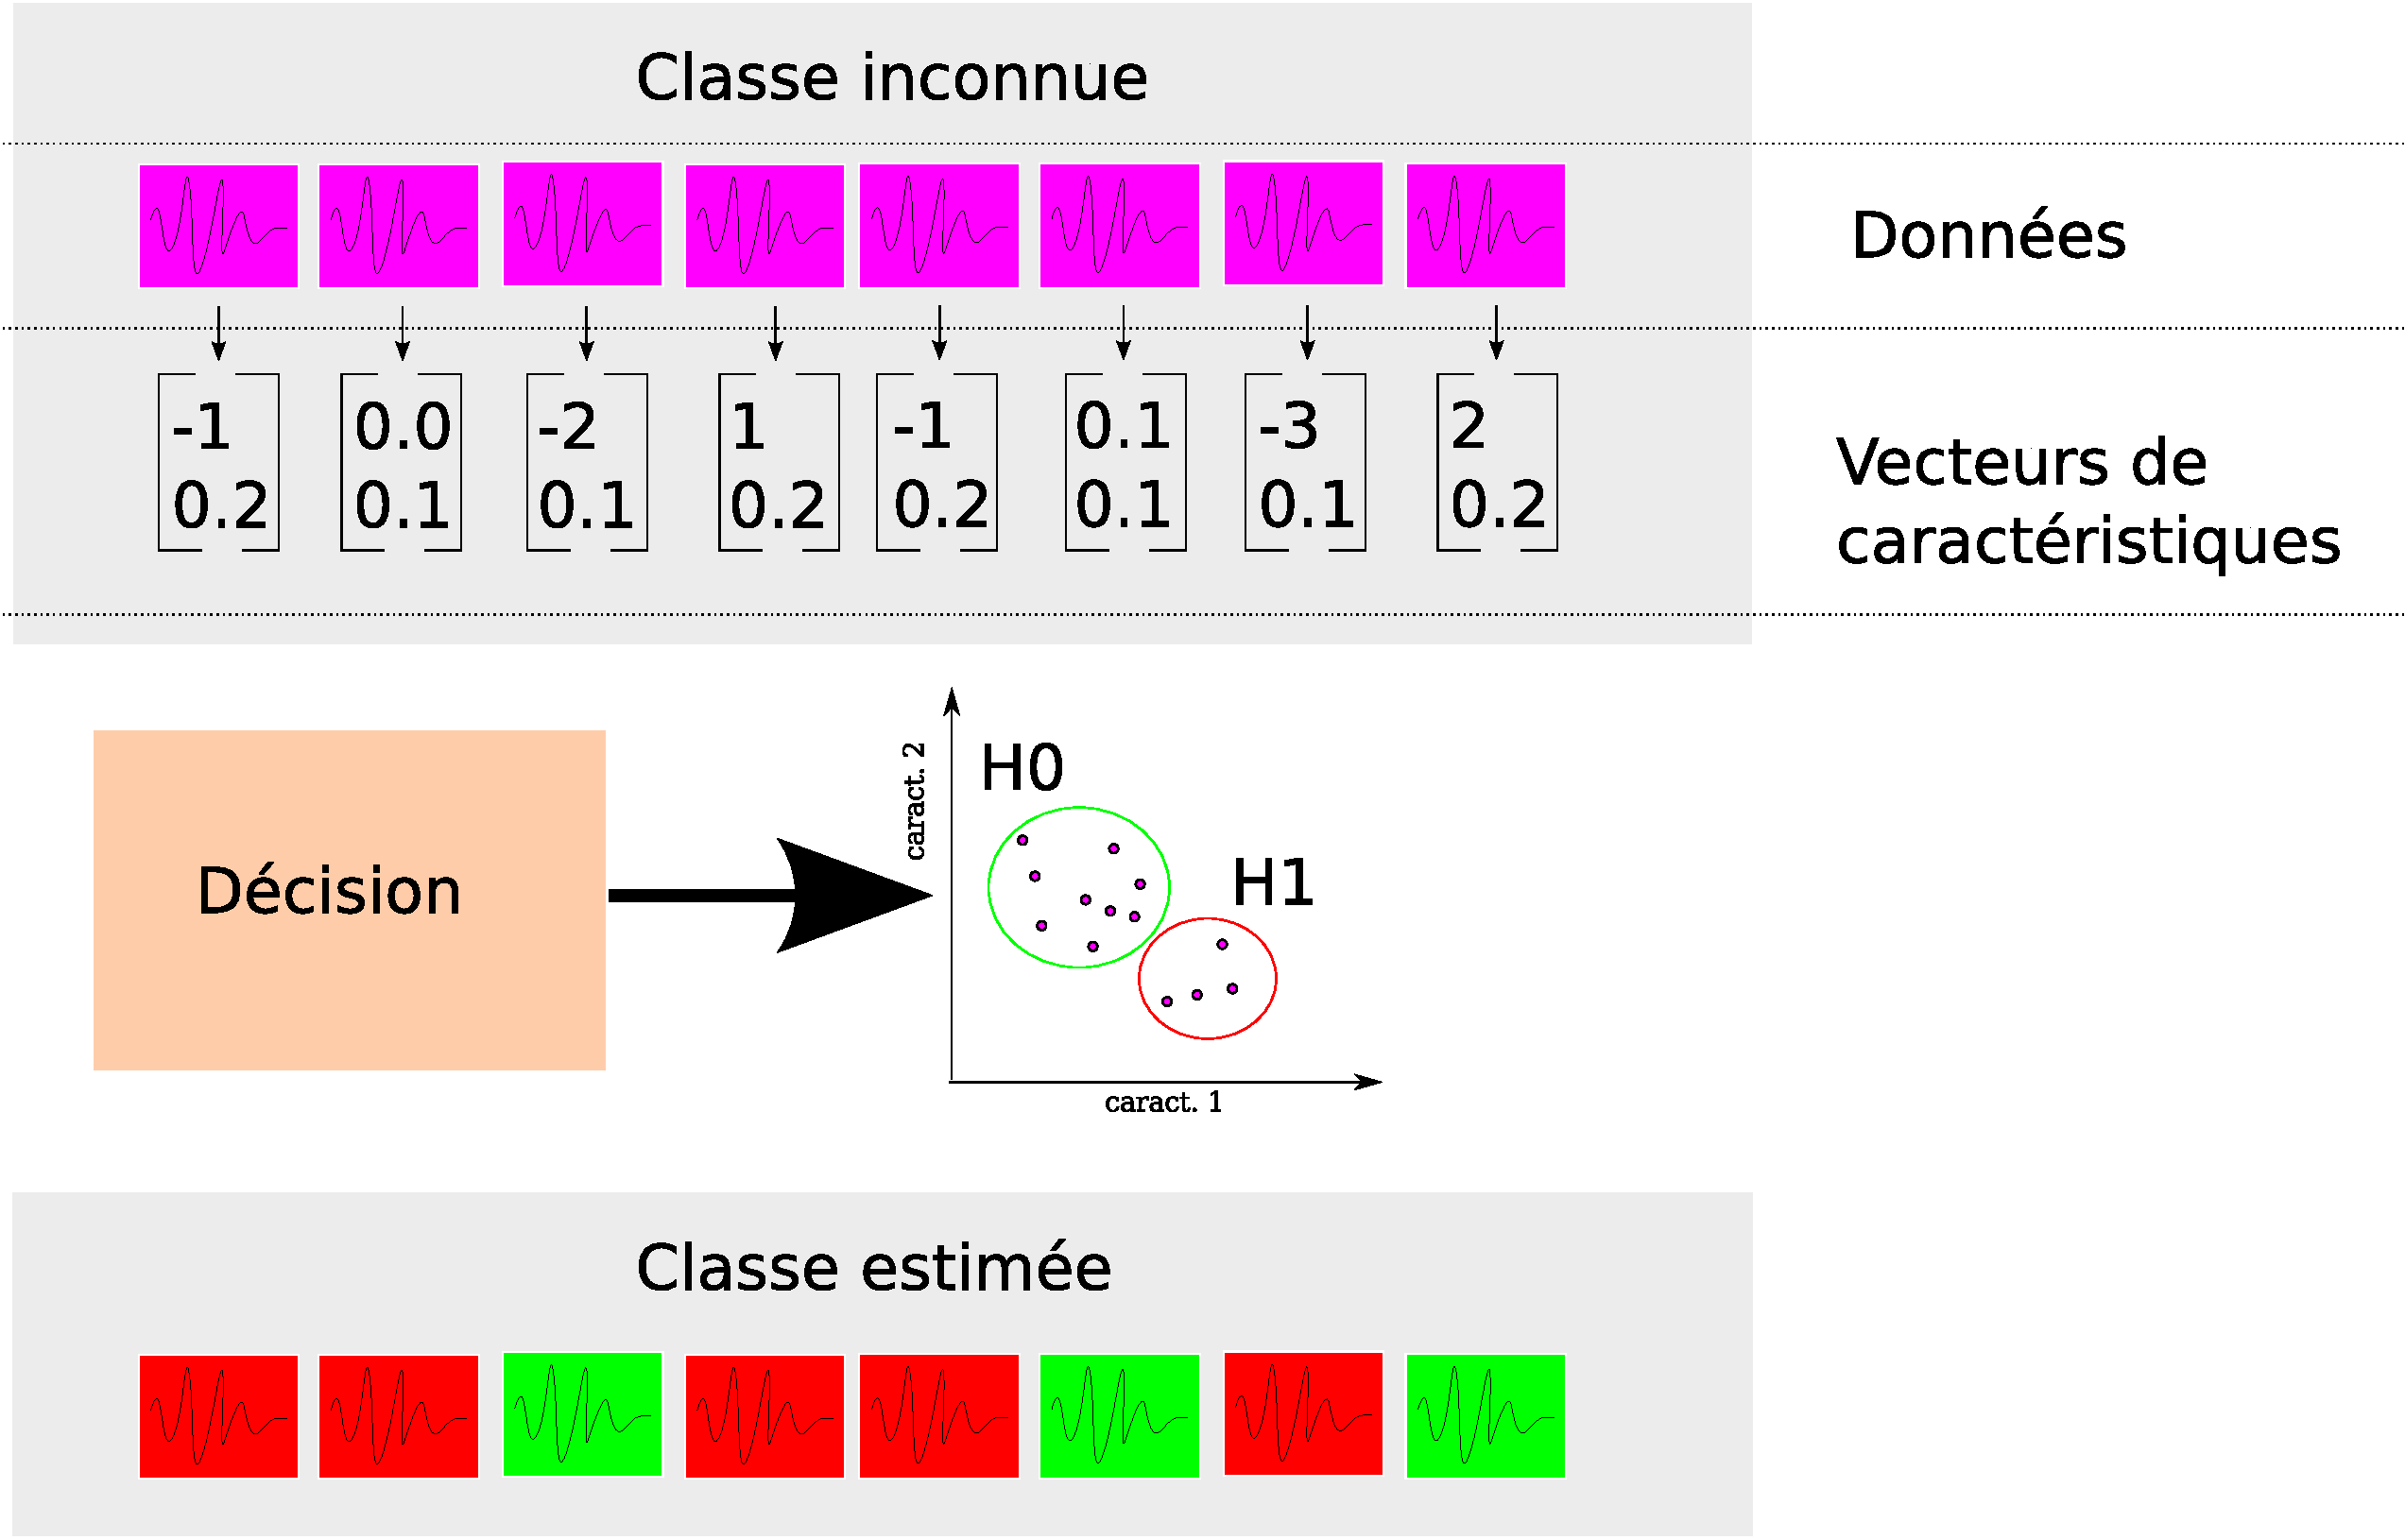
\includegraphics[width=15cm]{images/fonctionnementClassifNonSup}
	\end{center}
	\caption[Fonctionnement d'un classifieur non supervisé]{Fonctionnement d'un classifieur non supervisé : Les données brutes sont envoyées au classifieur qui va les regrouper en classes en fonction de leur répartition dans l'espace des caractéristiques.}
	\label{fig:fonctionnementClassifNonSup}
\end{figure}


		\subsection{Méthodes supervisées}

La classification supervisée vise à étiqueter des observations à partir de connaissances acquises \textit{a priori}.

Les classifieurs supervisés nécessitent une connaissance \textit{a priori} des classes. On entraîne le classifieur en lui fournissant des \emph{exemples} de cas avec l'étiquette associée. A partir de cette base de données d'entraînement, le classifieur va générer un \emph{modèle} prédictif permettant de classer de futurs exemples non encore connus, comme présenté dans la figure~\ref{fig:fonctClassif}.

\begin{figure}[h]
	\begin{center}
	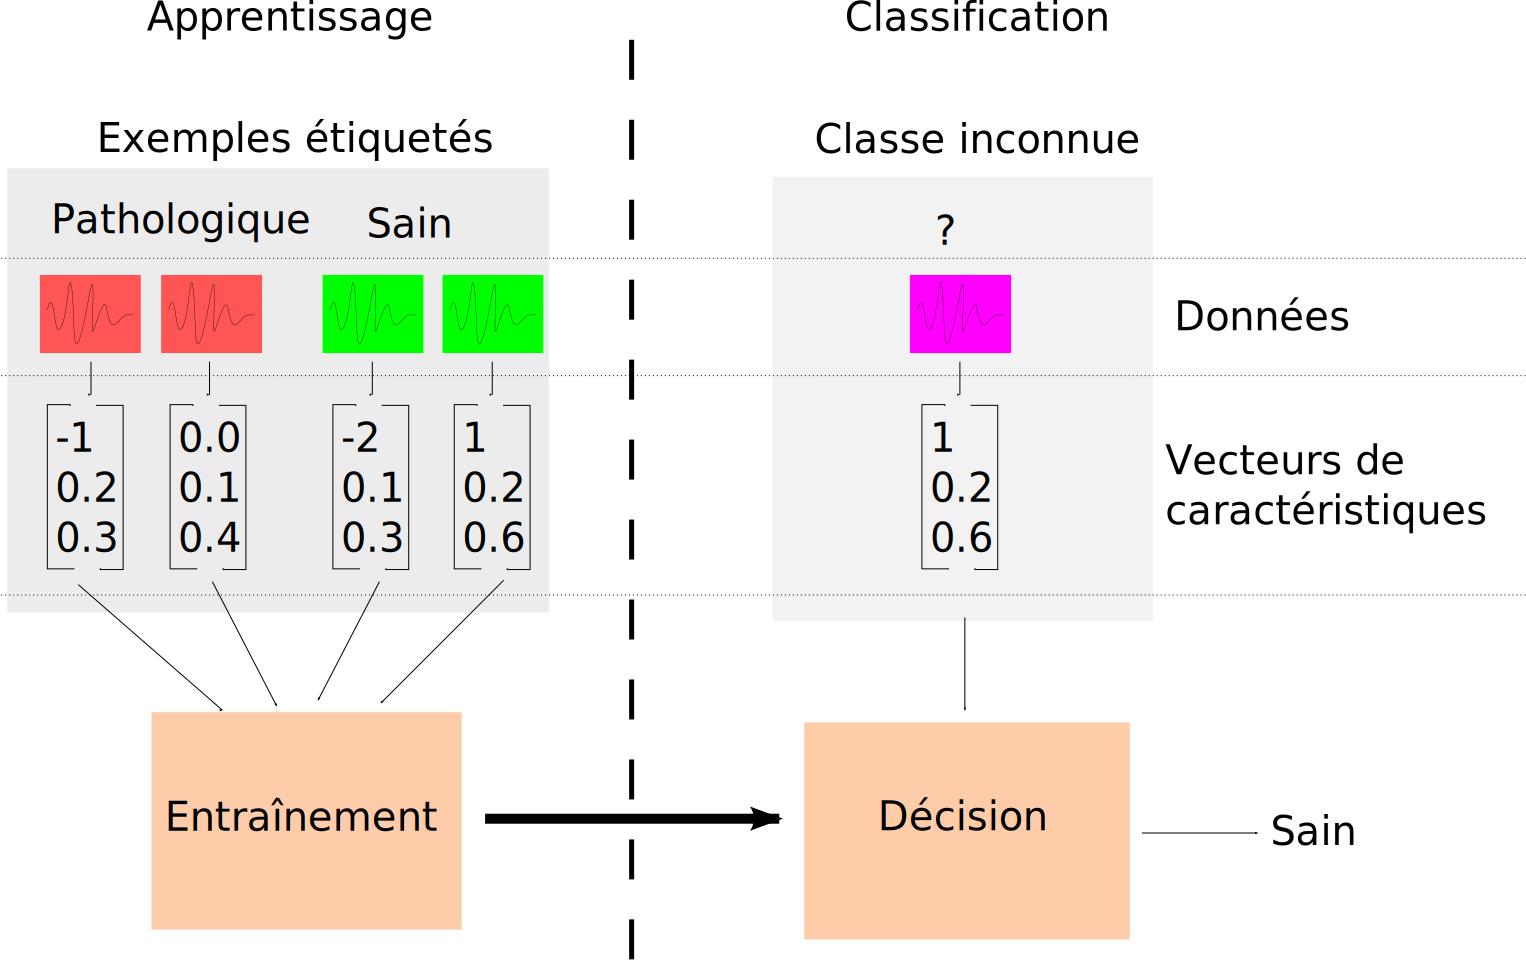
\includegraphics[width=15cm]{images/fonctionnementClassif}
	\end{center}
	\caption[Fonctionnement d'un classifieur supervisé]{Fonctionnement d'un classifieur supervisé : Les données d'apprentissage servent à entraîner le classifieur pour générer un modèle. Ce modèle permettra de rattacher des observations aux classes apprises.}
	\label{fig:fonctClassif}
\end{figure}


	\section{Machines à vecteur de support (SVM)}

\label{lab:SVM}
La ``Machine à Vecteur de Support'', aussi appelée ``Séparateur à Vaste Marge'', ou ``Support Vector Machine'' en Anglais, est un classifieur qui comme son nom l'indique vise à maximiser la marge~\cite{boser1992training}, qui est la distance minimale entre les points des données et la surface séparatrice (voir figure~\ref{fig:SVM}).

\begin{figure}[h]
	\begin{center}
	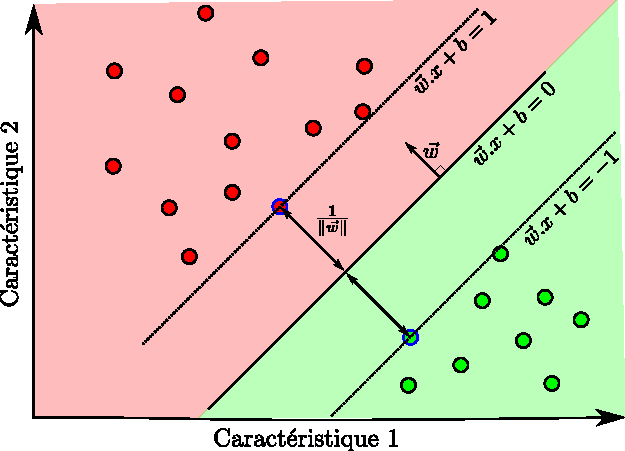
\includegraphics[width=12cm]{images/SVM}
	\end{center}
	\caption[Machine à Vecteur de Support]{Machine à Vecteur de Support : les points vecteur de support (entourés de bleu) sont les seuls utilisés pour calculer la surface de séparation d'équation $w . x + b = 0$. Le vecteur $w$ est normal à la surface de séparation et permet de calculer la marge $\frac{1}{\Vert w \Vert}$.}
	\label{fig:SVM}
\end{figure}


Les SVM sont des classifieurs supervisés qui cherchent à maximiser la séparation entre chaque classe. L'idée sous-jacente aux SVM est de trouver l'hyperplan optimal de séparation, et non pas n'importe quel hyperplan qui permettrait de séparer correctement les données d'apprentissage (figure~\ref{fig:multiPlansSeparationSVM}). 


\begin{figure}[h]
	\label{fig:multiPlansSeparationSVM}
	\begin{center}
	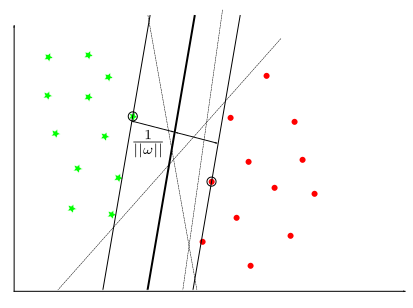
\includegraphics[width=13cm]{images/multiPlansSeparationSVM}
	\end{center}
	\caption[Illustration du principe d'optimisation de la marge sur le SVM]{Illustration du principe d'optimisation de la marge sur un cas à deux classes et deux caractéristiques : Il existe une infinité d'hyperplan qui séparent correctement les classes ``étoile vertes'' et ``ronds rouges'', représentés par les traits fins en pointillé. Cependant, il existe seulement une seule solution qui maximise la marge. Cette solution est représentée en trait plein, avec la marge $\frac{1}{||w||}$. Les points entourés en noir sont les points support utilisés pour contraindre l'hyperplan. }
\end{figure}


La définition de la marge et de l'hyperplan se fait à partir des vecteurs de support. Ils correspondent aux cas extrêmes des deux classes qui pourraient éventuellement poser des problèmes de classification.


Soit $\{(x_i, y_i) | x_i \in \mathbb{R}^p , y_i \in \{ -1, 1 \} \}$ un ensemble de points étiquetés correspondant à la base d'apprentissage. $x_i$ correspond au vecteur caractéristique, tandis que $y_i$ correspond à la classe du point.

Tout hyperplan dans l'espace des caractéristiques $\mathbb{R}^p$ peut être écrit $w . x - b = 0$, avec $w$ la normale à l'hyperplan et $\frac{b}{ ||w|| }$ le décalage de l'hyperplan par rapport à l'origine. 

La contrainte principale sur $w$ et $b$ est de classer correctement les données. Pour cela, les points vecteur de support devront respecter la contrainte $y_i ( w . x_i - b ) >= 1$. Par construction, les vecteurs de support correspondent aux points où l'égalité stricte est observée : $y_i ( w . x_i - b ) = 1$, comme indiqué sur la figure~\ref{fig:SVM}.

La seconde contrainte est la maximisation de la marge, qui correspond à  $\frac{2}{||w||}$, ce qui revient à minimiser $||w||$ comme indiqué sur la figure~\ref{fig:multiPlansSeparationSVM}.

La solution de ce problème d'optimisation est apportée par l'algorithme des multiplicateurs de Lagrange. 

Cependant, il peut arriver que les classes ne soient pas séparables. Ce problème est résolu par l'autorisation d'une erreur~\cite{cortes1995support} $\xi_i$  que l'on cherchera à minimiser : $( w . x_i - b ) >= 1 - \xi_i $. Cela engendre l'ajout d'un paramètre noté $C$, qui sera utilisé dans le lagrangien pour pénaliser plus ou moins les erreurs.

Dans le cas où l'hyperplan de séparation ne pourrait pas être défini par une équation linéaire, des fonctions à noyaux sont utilisées pour projeter les points dans un espace de plus grande dimension où le problème devient linéaire (voir figure~\ref{fig:kernelTrick}). Cependant, la transformation n'est jamais réalisée explicitement car en pratique, le changement de dimension est utilisé uniquement lors de la comparaison entre les points. On utilise donc des fonctions de comparaison modifiées, appelées noyaux. Le noyau le plus couramment utilisé est le RBF (fonctions à base radiale) qui a un espace d'arrivée de dimensions infinies, ce qui est rendu possible par le fait que l'on ne réalise par la transformation directement, mais qu'elle est réalisée implicitement lors de la comparaison des points à l'aide de l'équation suivante :

\begin{equation}
k(x_i,x_j)=e^{-\gamma||x_i-x_j||^2}  
\end{equation}

\begin{figure}[h]
	\begin{center}
	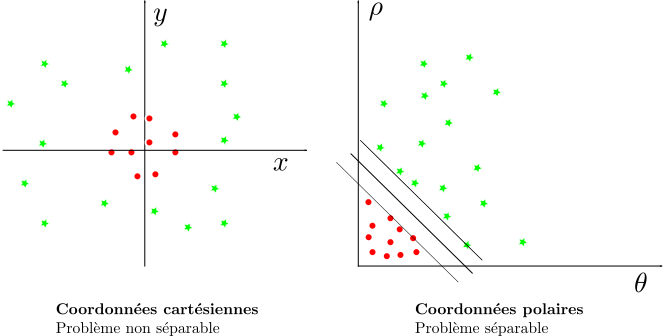
\includegraphics[width=15cm]{images/kernelTrick}
	\end{center}
	\caption[Changement de base pour les SVM]{Illustration du principe du changement de base : Des données non séparables dans le repère original peuvent devenir séparables en utilisant les noyaux. Dans ce cas, le passage des coordonnées cartésiennes aux coordonnées polaires permet de rendre le problème original linéairement séparable.}
	\label{fig:kernelTrick}
\end{figure}


Grâce à la maximisation de la marge, les SVM sont performants dans le cas où l'on ne dispose que de faibles quantités de données. D'autres algorithmes tels que les forêts aléatoires parviennent à obtenir des performances similaires~\cite{statnikov2008comprehensive}.

\subsection{Autres classifieurs supervisés}

De nombreux classifieurs supervisés ont été développés :

\label{lab:LDA}
Le classifieur LDA~\cite{fisher1936use} approxime les deux classes en supposant qu'elles ont une distribution gaussienne de covariance égale. Seule la moyenne de chaque distribution varie, et tout nouveau point est classé en fonction de sa distance à l'une ou l'autre des classes. Bien qu'il soit très rapide, ce classifieur ne fonctionne que dans le cas linéaire. L'approximation gaussienne donne des résultats suffisament bons dans de nombreux cas, ce qui explique son utilisation pour la détection des lésions en mammographie~\cite{baydush2007incorporation} ou en oncologie TDM~\cite{gurcan2002lung}.


Les réseaux de neurones~\cite{haykin1999neural} sont des classifieurs non linéaire qui se basent sur un fonctionnement simplifié des neurones du cerveau humain. il sont constitués de neurones artificiels qui miment les réactions des neurones biologiques. Un neurone applique une fonction à la combinaison linéaire de ses stimuli d'entrée. Chaque élément du vecteur de caractéristique est entré dans un neurone, qui ira stimuler un ou plusieurs autres neurones. L'information se propage jusqu'à un neurone terminal qui donnera le résultat. Les réseaux de neurones sont très performants, mais souffrent de difficultés de mise en place à cause de leur grand nombre de paramètres et de temps d'apprentissage très importants.

Une forêt de décision est un classifieur relativement récent basé sur plusieurs arbres de décisions initialisés différemment~\cite{ho1998random}. Le résultat de ce classifieur est le mode des résultats de tous les arbres. La combinaison de plusieurs arbres différents permet d'améliorer la stabilité du classifieur, qui est un gros désavantage des arbres de décision pris indépendamment. Ce classifieur est très rapide et très performant.